\section{A receptor based model for hydra morphogenesis}

\subsection{Introduction of the model}

\subsubsection{Biological derivation and description of kinetics}
We put ourselves in the following scenario: Epithelial cells continuously produce receptors, ligands and enzymes. At first, receptors are in an unbound state and are called \textit{free receptors}. When a \textit{ligand} reversibly binds to a free receptor, the pair is then called \textit{bound receptor}. Similarly, an interaction between an \textit{enzyme} and ligand results in the destruction of the ligand. We consider the space $\Omega$ to be a closed medium in which molecules can meet and interact (see \ref{phy_stat} for a schematic representation of the situation). 
\begin{figure}
	\label{phy_stat}
	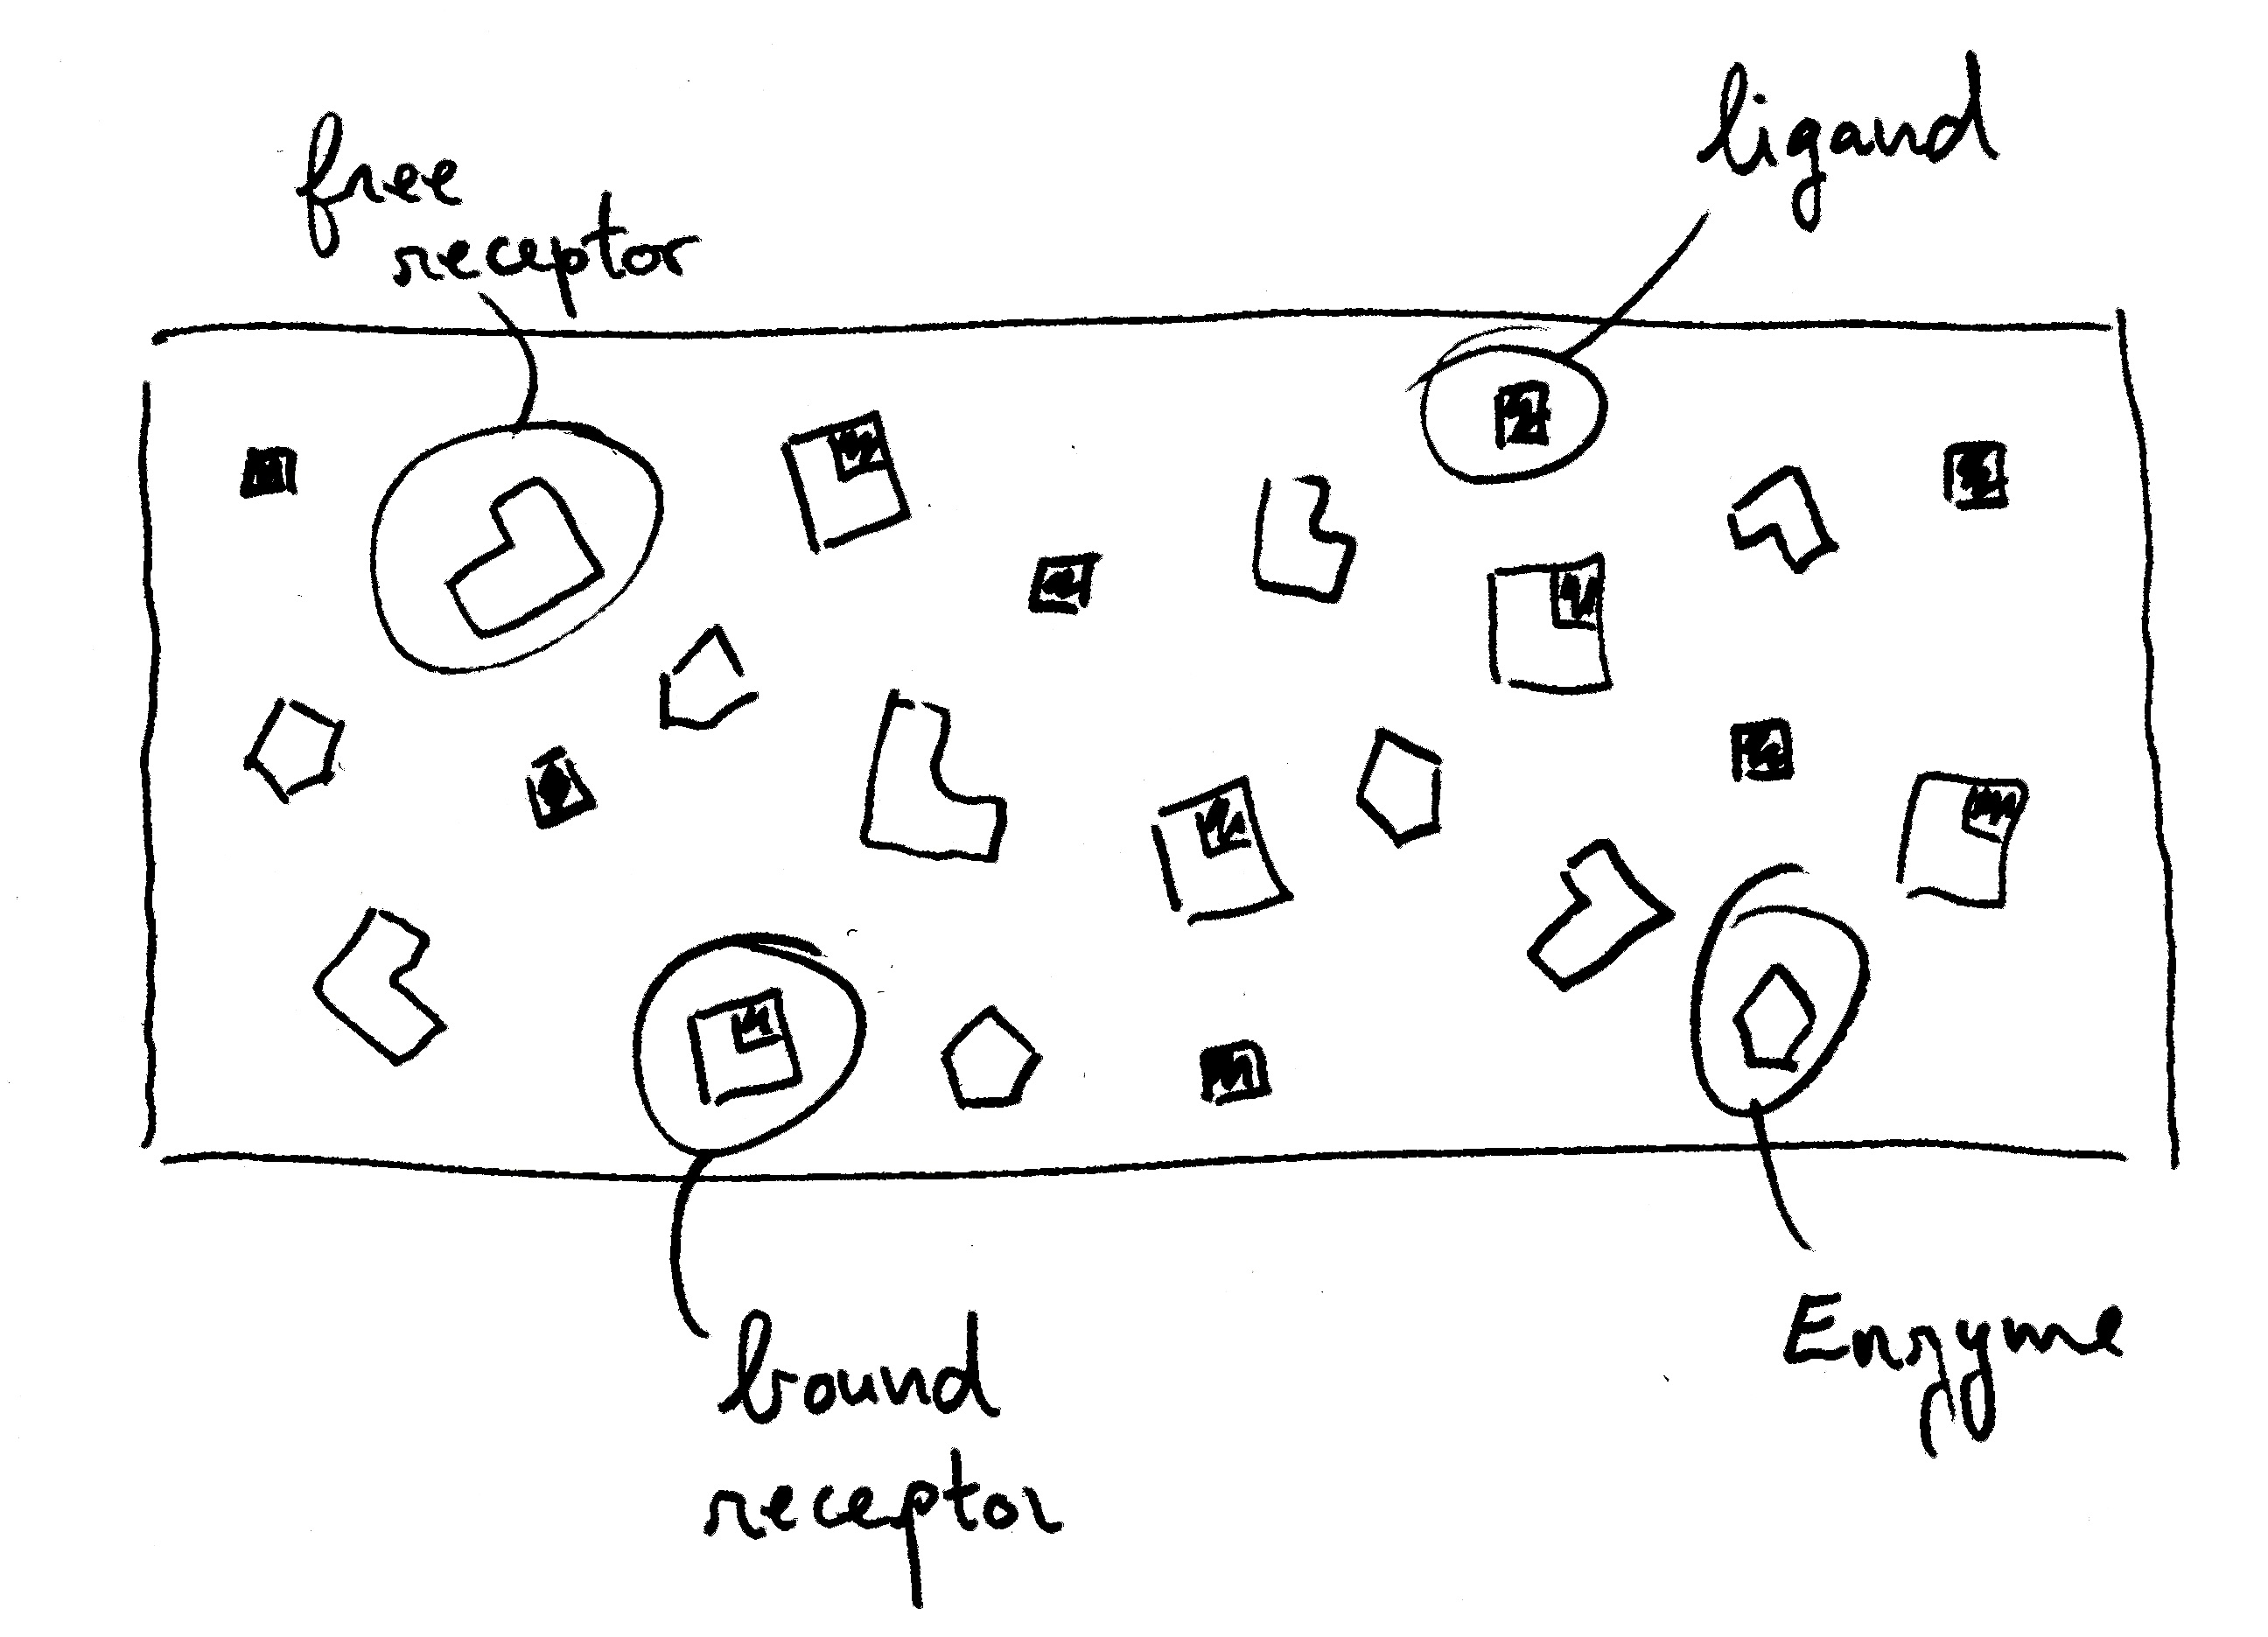
\includegraphics[width=\linewidth, height=8cm]{figures/epi_scheme.jpeg}
	\caption{Maybe replace with a tikz figure to have things look cleaner}
\end{figure}
Additionally, we assume that both ligands and enzymes are subject to molecular diffusion while free (and bound) receptors are not. Let 
$$r_f := \frac{\hash \text{free receptors}}{|\Omega|}, \quad r_b := \frac{\hash \text{bound receptors}}{|\Omega|}, \quad l := \frac{\hash \text{ligands}}{|\Omega|}, \quad e := \frac{\hash \text{enzymes}}{|\Omega|},$$
denote the concentration of each molecule. We use methods from chemical kinetics and statistical physics to infer equations describing the reaction.

All binding processes (receptors-ligands, ligands-enzymes) are assumed to be governed by the law of mass action kinetics.  Free receptors, ligands and enzymes are produced by epithelial cells at rate $p_r, p_l, p_b$ and degraded at rates $\mu_r, \mu_l, \mu_e$. On the other hand bound ligands are internalized by the cell at rate $\mu_b$. Binding and dissociation rates between ligands and receptors are denoted by letters $b$ and $d$. Enzymes bind to ligands with rate $b_e$, leading to the destruction of said ligands. And finally, we let $D^l$ and $D^e$ denote the diffusion rates of ligands and enzymes respectively. Altogether, we end up with the following set of equations

\begin{align}
\del_t r_f &= -\mu_f(r_f) + p_r(r_f, r_b) - b(r_f, l) + d(r_b) \label{eq:kinrf}\\[0.5em]
\del_t r_b &= - \mu_b(r_b) + b(r_f, l) - d(r_b) \label{eq:kinrb}\\[0.5em]
\del_t l &= \eps d_1 \del_x^2 l - \mu_l(l) - b(r_f, l) + p_l(r_f, r_b) +d(r_b) - b_e(l, e) \label{eq:kinl}\\[0.5em]
\del_t e &= \eps d_2 \del_x^2 e - \mu_e(e) + p_e(l, r_b) \label{eq:kine}
\end{align}

Supplemented with homogeneous Neumann boundary conditions on $\Omega = (0, L)$ (which physically represents a one-dimension sheet of epithelial cells along the body column). 


\begin{figure}
	\label{diagram}
	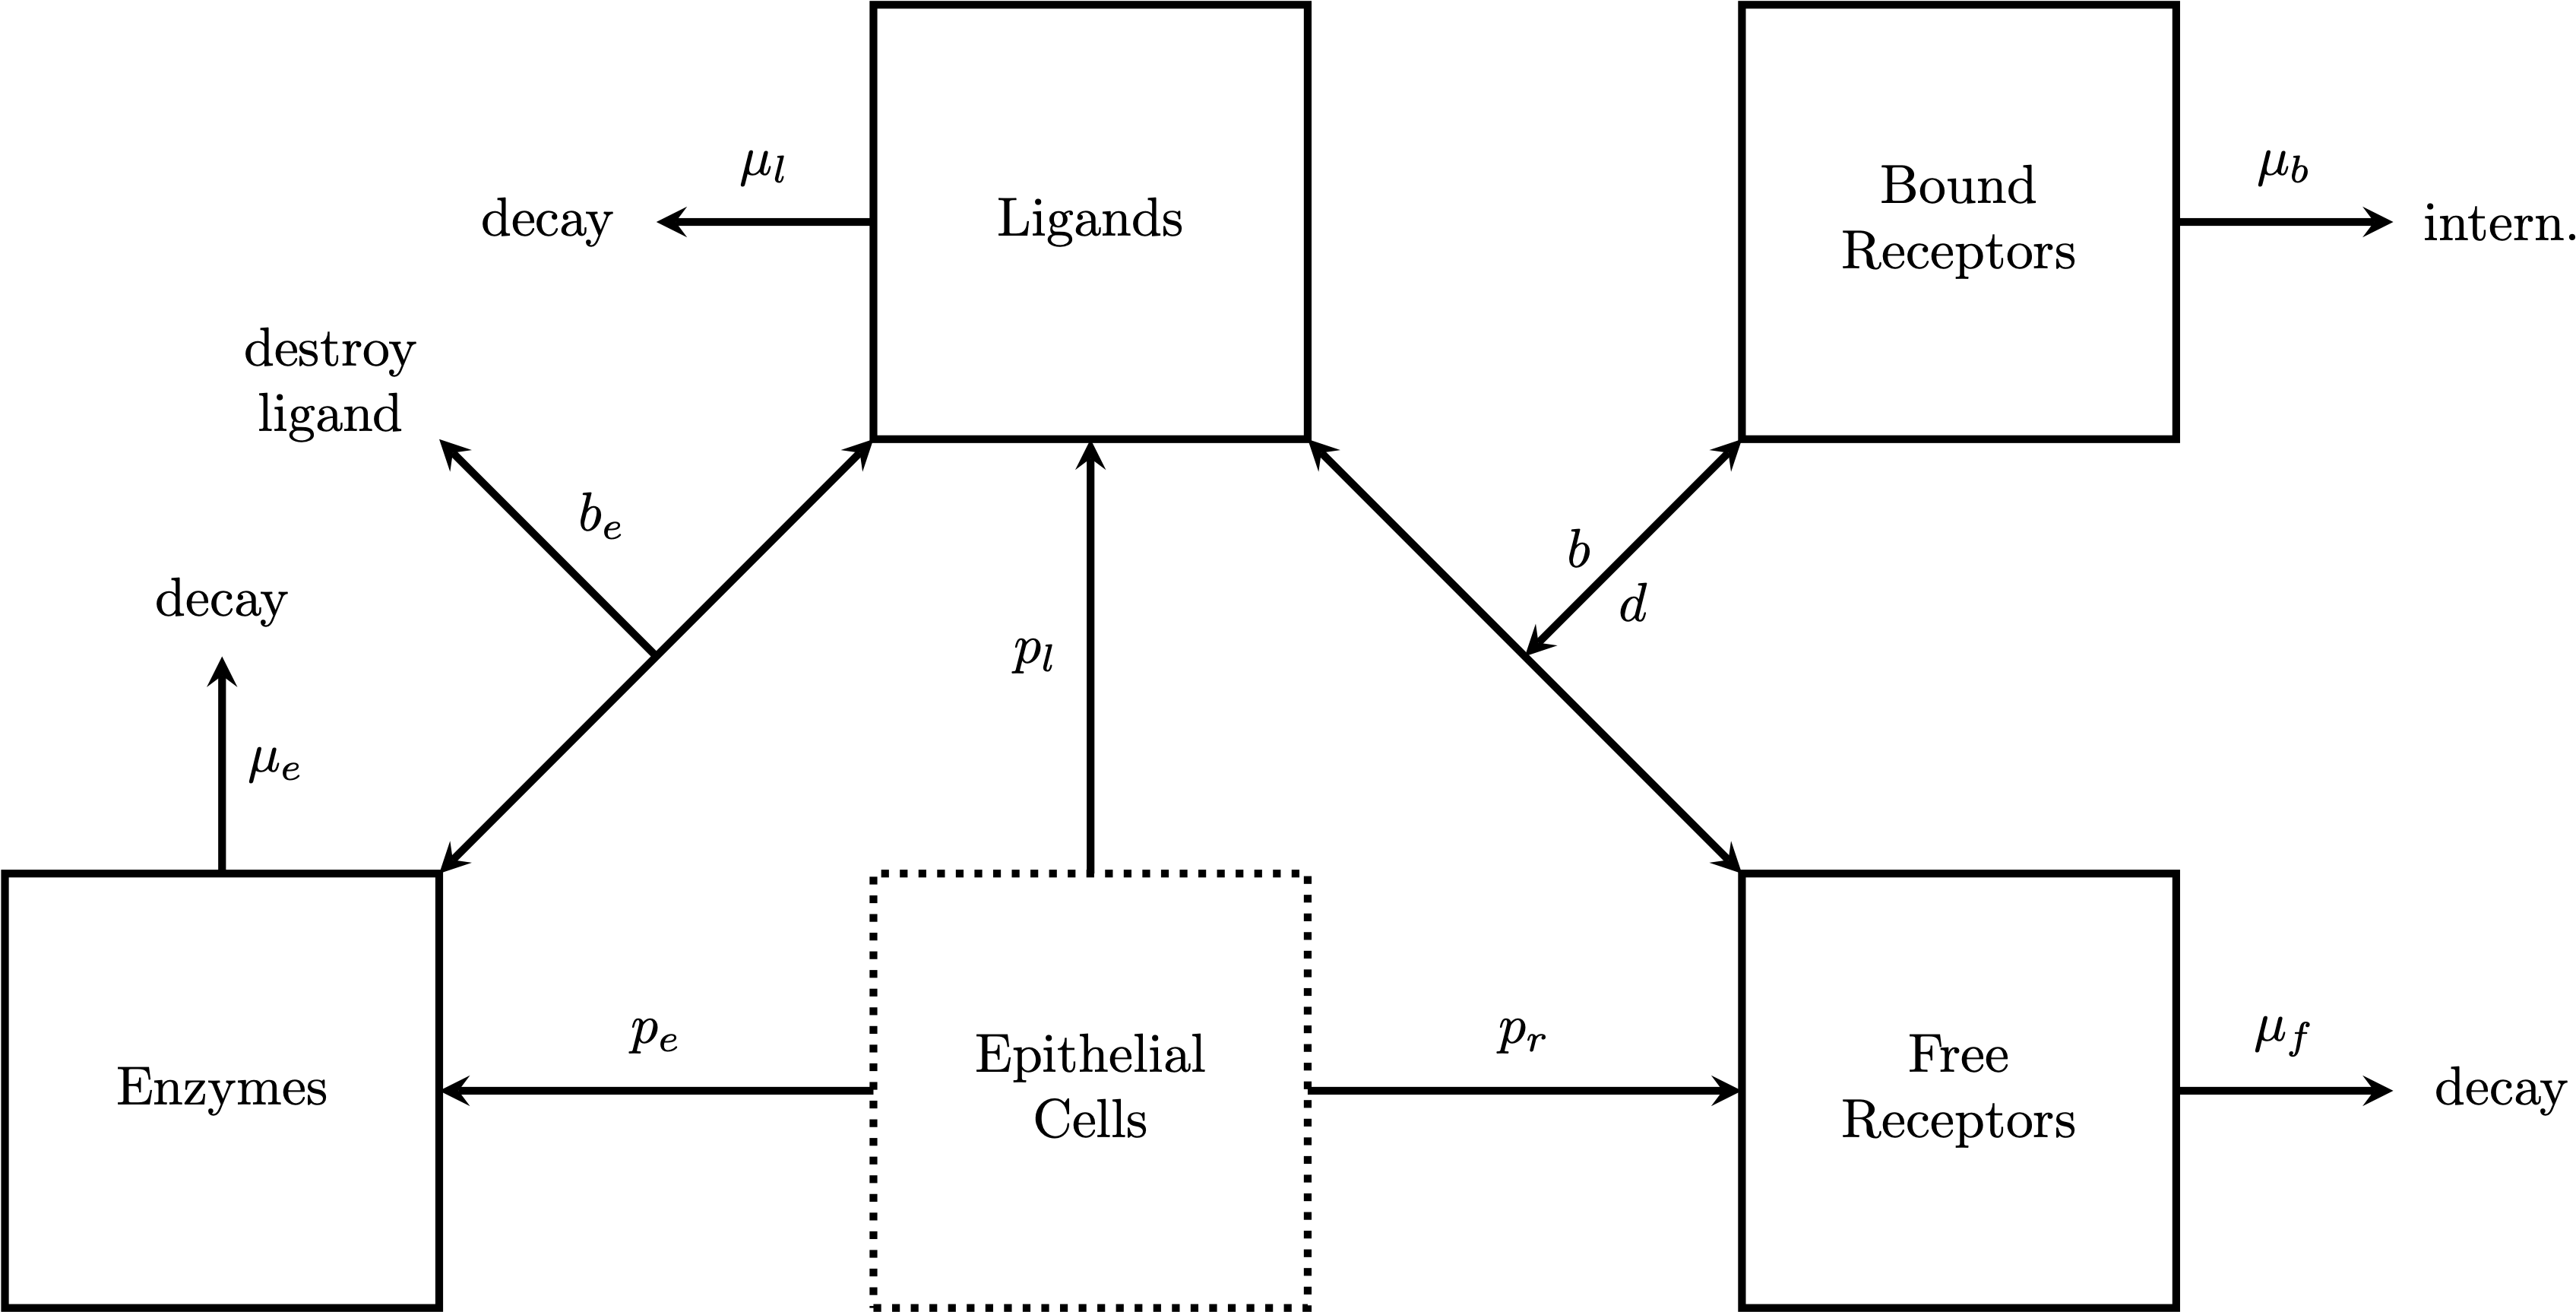
\includegraphics[width=\linewidth]{figures/DIAGRAM_MODEL.png}
	\caption{Diagram representation of the model}
\end{figure}

\subsubsection{Choosing kinetic functions}

Again in \cite{AnnaThesis}, two choices of kinetics are explored to study (\ref{eq:kinrf})-(\ref{eq:kine}). Some results can be proved about the model in the general case with weak assumptions on each functions, but then we cannot make use of numerics to get a visual grasp of the situation. This is why we decide to define each function in the model using one of the choices in \cite{AnnaThesis} (and keep the other one as an extension for further researches). In what follows, we define every rates $b, d, b_e, \mf, \mb, \ml, \me$:

\begin{center}
	\begin{tabular}{c >{\hspace{5em}} c}
		$b(r_f, l) = b r_f l$ & $b \in \R_{>0}$ \\[0.5em]
		$b_e(l, e) = b_e l e$ & $b_e \in \R_{>0}$ \\[0.5em]
		$d(r_b) = d r_b$ & $d \in \R_{>0}$
		\\[0.5em]
		$\mf(r_f) = \mf r_f$ & $\mf \in \R_{>0}$ \\[0.5em]
		$\mb(r_b) = \mb r_b $ & $\mb \in \R_{>0}$ \\[0.5em]
		$\ml(l) = \ml l$ & $\ml \in \R_{>0}$
		\\[0.5em]
		$\me(e) = \me e$ & $\me \in \R_{>0}$
	\end{tabular}
\end{center}
And the production rates are the same given by Michaelis-Mentel-like reaction terms 

\begin{center}
	\begin{tabular}{r >{\hspace{5em}} c}
		$p_r(r_f, l) = m_1\dfrac{r_b}{1 + r_b}$ & $m_1 \in \R_{>0}$ \\[1em]
		$p_l(l, e) = m_2\dfrac{r_b}{1 + r_b}$ & $m_2 \in \R_{>0}$ \\[1em]
		$p_e(r_b) = m_3\dfrac{r_b}{1 + r_b}$ & $m_3 \in \R_{>0}$
	\end{tabular}
\end{center}


\subsection{Model reduction and properties}

The system of PDE defined in (\ref{eq:kinrf})-(\ref{eq:kine}) has been extensively studied in \cite{AnnaThesis}. It has been shown that such a model can exhibit Turing patterns under some conditions on the Jacobian of the linearized system. In this thesis, we proceed in a similar fashion, but there is a twist. The next paragraphs are dedicated to reducing the model using quasi-steady-state approximation and re-parametrization.

\subsubsection{Quasi-steady-state approximation}

The Quasi-Steady-State Approximation (QSSA) is a  technique inspired from the field of  chemical kinetics or more generally biochemistry. When introduced, the purpose of such an approximation is to simplify the analysis by assuming that certain chemical species are reaching their steady-state concentrations quicker than other species in the system.

First used in an \textit{ad hoc} fashion by biologists, they theory behind QSSA has been thoroughly explored and is now carefully described thanks to the framework provided by singular perturbation theory. This approach turns out to be particularly efficient for equations emerging from chemistry. When performing QSSA, the rate of change of concentrations of these slower species is assumed to be negligible compared to the rates of other reactions in the system. Therefore, the concentrations of these species can be approximated as constants during the time course of the reaction.

\begin{remark}
Although the QSSA can be proven to be physically relevant when applied to some systems (e.g., it works in our case \com{maybe prove it if time ?}), the approximation may not always hold true under certain conditions.
\end{remark}

Coming back to our system, we perform a QSSA on the quantity $r_b$, \textit{i.e.}, we assume $\del_t r_b = 0$. and find $(d + \mu_b) r_b = b u v $ from substituting the value of $\del_t r_b$ by 0 in (\ref{eq:kinrb}) and solving for $r_b$. Some rearranging yields

$$r_b = \dfrac{b}{d + \mu_b} u v.$$

From now on, we let $\alpha = b / (d + \mu_b)$ and replace the newly found value of $r_b$ in (\ref{eq:kinrf})-(\ref{eq:kine}):

\begin{align}
    \del_t u &= -\mu_f u + m_1 \dfrac{\alpha u v}{1 + \alpha u v} - b u v + d \alpha u v, \label{eq:kinu} \\[0.5em]
    \del_t v &= \eps d_1 \del_x^2 v - \mu_l v + m_2 \dfrac{\alpha u v}{1 + \alpha u v} - b u v + d \alpha u v - b_e v w,  \label{eq:kinv}\\[0.5em]
    \del_t w &= \eps d_2 \del_x^2 w - \mu_e w + m_3 \dfrac{\alpha u v}{1 + \alpha u v}. \label{eq:kinw}
\end{align}

\subsubsection{Change of variable}

Now that we have reduced the amount of variables from four to three, let us also operate surgery on the system to get rid of some parameters. First, a quick computation shows that $d\alpha - b = -\mu_b \alpha$. Then, we introduce the set of new variables (and parameters) 

\begin{center}
\begin{tabular}{c>{\hspace{2em}} c<{\hspace{2em}} c<{\hspace{2em}} c<{\hspace{2em}}}
	$\Tilde{u} = \sqrt{\alpha} u$, & $\Tilde{v} = \sqrt{\alpha} v$, & $\Tilde{w} = b_e w$, & $\Tilde{\mu}_b = \sqrt{\alpha} \mu_b$,\\[1em]
	$\Tilde{m_1} = \sqrt{\alpha} m_1$, & $\Tilde{m_2} = \sqrt{\alpha} m_2$, & $\Tilde{m_3} = b_e m_3$,
\end{tabular}
\end{center}

which, once substituted back in equations (\ref{eq:kinu})-(\ref{eq:kinw}), yields the fully reduced system

\begin{align}
	\del_t \Tilde{u} &= -\mu_f \Tilde{u} + \Tilde{m}_1 \dfrac{ \Tilde{u} \Tilde{v}}{1 +  \Tilde{u} \Tilde{v}} - \Tilde{\mu_b} \Tilde{u} \Tilde{v} \label{eq:redu}, \\[0.5em]
	\del_t \Tilde{v} &= \eps d_1 \del_x^2{\Tilde{v}} - \mu_l  \Tilde{v} +\Tilde{m}_2 \dfrac{\Tilde{u} \Tilde{v}}{1 +  \Tilde{u}\Tilde{v}} - \Tilde{\mu_b} \Tilde{u} \Tilde{v} - \Tilde{v} \Tilde{w}, \label{eq:redv} \\[0.5em]
	\del_t \Tilde{w} &= \eps d_2 \del_x^2{\Tilde{w}} - \mu_e\Tilde{w} + \Tilde{m}_3 \dfrac{\Tilde{u}\Tilde{v}}{1 + \Tilde{u}\Tilde{v}}. \label{eq:redw}
\end{align}

For the sake of readability, we drop the $\sim$ notation in the future and let $\bm f = (f, g, h)$ denote the kinetic part of system (\ref{eq:redu})-(\ref{eq:redw}), i.e.: 
\begin{align}
	f(u, v, w) &= -\mu_f u + m_1 \dfrac{uv}{1 + uv} - \mu_b uv, \\
	g(u, v, w) &= -\mu_l v + m_2 \dfrac{uv}{1 + uv} - \mu_b uv - vw, \\ 
	h(u, v, w) &= -\mu_e w + m_3 \dfrac{uv}{1 + uv}.
\end{align}

This is the model we seek to investigate in this thesis. In coming sections, we prove that there exists solutions to the system for an arbitrary time $t>0$. A soon as existence of solutions is past us, we focus on the steady-states of the system based on the choice of parameters and perform a bifuraction analysis with respect to $\mu_b$. Finally, we focus on the linear stability using tools developed in section (SECTION GENERAL FRAMEWORK - LINEAR INSTABILITY) and move on to simulations.

\subsection{Existence of solutions}


In this section, we prove the global existence of solutions to system (\ref{eq:system}) using the theory established by Smoller in \cite{Smoller1994}. In this direction, we introduce the notion of invariant regions, invariant rectangles and $\bm\phi$-stability together with a few theorems that we use to reach our result. We already know from (theorem 14.4, \cite{Smoller1994}) that there exists local solutions to system (\ref{eq:system}) defined on a short interval $[0, \delta)$. Therefore, let us extend these local solutions to global solutions of the reaction-diffusion problem. First, we need

\begin{definition}[Invariant region, \cite{Smoller1994}]
	A closed subset $\Sigma \subset \R^n$ is called a (positively) invariant region for the local solution defined by 
	\be\label{eq:smoller_sys}\del_t \bm v = \varepsilon D \del_x^2 \bm v + M \del_x v + \bm \phi(v, t),\ee
	$$\bm v(x, 0) = v_0(x) \quad x\in\Omega,$$ 
	if any solution $\bm v(x, t)$ having all of its boundary and initial values in $\Sigma$, satisfies $\bm v(x, t) \in \Sigma$ for all $x\in\Omega$ and for all $t \in [0, \delta)$.
\end{definition}  

Notice that this results works for a more general class of equations than ours. Indeed, here, $\varepsilon = 1$, $D$ is a diagonal matrix with constant positive entries, $M=0$ and $\bm \phi$ is independent of time (system is autonomous). As far as we are concerned, all regions of interest can be described by the intersection of $(n-1)$-dimensional hypersurfaces 
\be\label{eq:sigma}\Sigma = \bigcap_{i \in \mathcal I} \{G_i \le 0 \},\ee
 where $G_i = G_i(u, v, w)$ are smooth, real-valued function defined on $\mathrm{Dom}(G_i) \supset \mathrm{im}(\bm u)$ such that $\grad G_i$ never vanishes for all $i \in \mathcal I$. In the special case where $\Sigma$ is invariant and generated by affine constraints ($G_i(\bm v) = \bm v - \alpha$, for some $\alpha \in \R$), $\Sigma$ is referred to as invariant rectangle. We also introduce

\begin{definition}[$\bm\phi-$stability \cite{Smoller1994}]
	A system of the form 
	\begin{equation}
		\label{rdsys}
		\del_t \bm v = D \del_{x}^2 \bm v + \bm \phi (v),
	\end{equation}
	 is said to be $\bm \phi-$stable if, whenever $\bm\phi$ is the limit of functions $\bm\phi_n$ in the $\mathcal C^1-$topology on compacta, for all $t>0$ then any solution of \ref{rdsys} supplemented with initial condition is the limit in the compact-open topology, of solutions of \ref{rdsys}, where $\bm\phi$ is replaced by $\bm\phi_n$ 
\end{definition}

Once again, taking into account the fact that our nonlinearities $\bm f$ are smooth, this general "regularity" statement allows us to use a stronger theorem with less points to verify in order to get global existence. The theorem is the following 

\begin{theorem}[Conditions for invariance, \cite{Smoller1994}]
	\label{thm:invariant_region}
	Let $\Sigma$ be defined as in (\ref{eq:sigma}), and consider the system \ref{eq:smoller_sys} with $M = 0$, $D$ positive definite and $\bm\phi = \bm\phi(\bm v, t)$. Suppose that this system is $\bm\phi$-stable. Then $\Sigma$ is a positively invariant region for \ref{eq:smoller_sys}) for fixed $\varepsilon > 0$ if and only if the following hold at each boundary point $\bm v_0$ of $\Sigma$ (so $G_i(\bm v_0) = 0$):
	
	\begin{itemize}
		\item[\textbf{a)}] $\grad G_i$ is a left eigenvector of $D$
		\item[\textbf{b)}] $G_i$ is quasi-convex at $\bm v_0$
		\item[\textbf{c)}] $\grad G_i(\bm \phi) \le 0$
	\end{itemize}
\end{theorem}

\begin{proof}
	See theorem 14.3 from \cite{Smoller1994}.
\end{proof}

Next, we will show that system (\ref{eq:system}) has an invariant rectangle $\Sigma$. It is $\bm f$-stable and our choice of constraints will always satisfy property \textbf{a)} from theorem \ref{thm:invariant_region}. The reason why is because we choose $G_i$ such that $\grad G_i$ is constant and has only one non-zero component. Therefore $\grad G_i$ will be a left eigenvector of $D$ with eigenvalue $d_{j}$ where $d_j$ is the $j$-th diagonal entry of $D$ and $j$ is the index where $\grad G_i$ is non-zero (notice that 0 can be an eigenvalue in our case). Since each $G_i$ is an affine constraint, it is naturally quasi-convex and it is therefore only left to verify \textbf{c)} to obtain the wanted result.


\begin{proposition}[Existence of an invariant rectangle]
	There exists three positive reals $A_u, A_v, A_w$ such that the region $$\Sigma = \bigl\{(u, v, w) : 0 \le u \le A_u, \quad 0 \le v \le A_v, \quad  0 \le w \le A_w, \bigr\},$$ is an invariant rectangle of system (\ref{eq:system})
\end{proposition}

\begin{proof}
	We start by writing $$\Sigma = \Sigma_0 \cap \Sigma_A =: \bigcap_i \biggl( \underbrace{\{G_\kappa \le 0\}}_{\Sigma_0} \cap \underbrace{\{H_\kappa \le 0\}}_{\Sigma_A}\biggr), \qquad \kappa = u, v, w.$$
	The rectangular region where each $G_i$ and $H_i$ are prescribing the constraints on $\Sigma$ defined as follows
	
	\begin{align*}
		& G_u(u, v, w) = -u & H_u(u, v, w) = u - A_u \\[1em]
		& G_v(u, v, w) = -v & H_v(u, v, w) = v - A_v \\[1em]
		& G_w(u, v, w) = -w & H_w(u, v, w) = w - A_w
	\end{align*}

	Each $G_i$ and $H_i$ is obviously smooth. Now For let $$\del\Sigma := \biggl\{(u,v,w) \in \Sigma : \exists i, \ \  G_i(u, v, w) = 0 \quad\text{or}\quad H_i(u, v, w) = 0 \biggr\},$$ be the boundary of $\Sigma$, we consider a point  $(u, v, w) \in \del \Sigma$ and proceed case-by-base. Let $X $ denote such a point, if $u=0$, then $$(\grad G_u \cdot \phi_f)(X)\bigl\vert_{u=0} = u \left( \mu_f  + \mu_b v - m_1 \dfrac{v}{1 + uv}\right)\biggl\vert_{u=0} = 0.$$ The case $v= 0$ is similar in a way that
	$$(\grad G_v \cdot \phi_f)(X)\bigl\vert_{v=0} = v \left( \mu_l  + \mu_b u + w - m_2 \dfrac{u}{1 + uv}\right)\biggl\vert_{v=0} = 0.$$ Finally, since $X \in \del\Sigma_0$, it holds that $u, v \ge 0$, meaning that if $w=0$, then $$(\grad G_w \cdot \phi_f)(X)\bigl\vert_{w=0} = -m_3 \dfrac{uv}{1 + uv} < 0.$$ We proceed in similar fashion to take care of $\del\Sigma_A$. First, we notice that
	
	\begin{align}
		f(u, v, w) &= -\mu_f + m_1 \dfrac{uv}{1 + uv} - \mu_b uv \notag \\[0.5em]
		& \le m_1 - \min(\mu_f, \mu_b) u (1 + v). \notag
	\end{align}
	
	Using the fact that $X \in \Sigma$, we deduce $1 + v \ge 1$ and therefore we get rid of it in the product, leaving us with 
	$$f(u, v, w) \le m_1 - \min(\mu_f, \mu_b) u.$$
	In other words, we can find $A_u \in \R_{>0}$ satisfying $A_u > m_1 / \min(\mu_f, \mu_b)$. This implies $(\grad H_u \cdot \phi_f)(X)\vert_{u=A_u} = f^1(A_u, v, w) \le 0$. The same logic applies to show $$g(u, v, w) \le m_2 - \min(\mu_f, \mu_b, 1) v.$$ Thus, by picking $A_v \ge m_2 / \min(\mu_f, \mu_b, 1)$, we get $(\grad H_v \cdot \phi_f)(X)\vert_{v=A_v} \le 0$. Finally, we show that $$h(u, v, w) \le m_3 - \mu_e w,$$ and take $A_w \ge m_3 / \mu_e$ to obtain $(\grad H_w \cdot \phi_f)(X)\vert_{w=A_w} \le 0$. Applying Theorem 3.16 from \cite{AnnaThesis} concludes the proof.
\end{proof}

We have thus proved the existence of an invariant rectangle. We finally use theorem 14.9, \cite{Smoller1994} to deduce the existence of the solution to (\ref{eq:system}) for all $t>0$ provided we take initial data $u_0$ continuous, bounded with values $u_0(x) \in \Sigma$ for $x \in \Omega$. This results can be extended to uniquely bounded initial conditions $u_0$ but the proofs and tools used are out of the scope of this thesis. Knowing we are now capable of guarantying the existence of a global solution under reasonable assumptions on our model, we can move to the analysis of steady-states.


